\section{Introduction}

%Intro
The Large Hadron Collider (LHC) was designed to operate at high design luminosities, enabling the study of physical phenomena with extremely small cross-sections \cite{CERN:lhc-design-report}. To achieve such a luminosity, protons are accelerated to an energy of \SI{6.8}{\tera\electronvolt}, grouped into bunches in opposing beams which cross one another every \SI{25}{\nano\second} \cite{CERN:lhc-run3-operation}. Capturing the detail of proton-proton (pp) collisions at a rate of \SI{40}{\mega\hertz} introduces an immense data challenge, in which recording collisions in full detail at a typical LHC experiment would require transferring and writing data at up to ${\sim}\SI{40}{\tera\byte\per\second}$. To reduce this data flow, High Energy Physics (HEP) experiments employ trigger systems: computing systems designed to perform detector readout, selection, calibration, etc. Typically $\mathcal{O}\left(\SI{1}{\giga\byte\per\second}\right)$ of data useful to the physics goals of an experiment is extracted.

Each LHC experiment discussed in this paper—ALICE, ATLAS, CMS and LHCb—has undertaken considerable research and development in the field of triggers and data acquisition (TDAQ). Developments in computational resources (e.g., the adoption of hybrid architectures) and data processing approaches (e.g., real-time and parallelised software frameworks) have enabled more advanced trigger systems to be developed in recent years. ALICE and LHCb performed significant upgrades to their trigger systems ahead of Run~3 of the LHC (2022-2025), with ATLAS and CMS planning upgrades of similar scales ahead of the High-Luminosity LHC (HL-LHC) operational period (2029-2040s). In this paper, the current trigger state-of-the art is reviewed, predominantly within the context of Run~3.

% Overview of trigger strategies
% Model detector, what does a non-specific trigger look like?
\subsection{Principles of triggering in High Energy Physics}

The primary function of a trigger system, as laid out in Figure~\ref{trigger-schema}, is to reduce the data rate an experiment must process without impairing the physics performance of the experiment \cite{Jeitler_2017, Smith2020, Beck_2007, ellis2010trigger}. The performance of a trigger system is therefore determined by the optimisation of three quantities: high signal efficiency, high background rejection (or equivalently low background efficiency) and affordable throughput/output bandwidth. To satisfy these requirements, triggers are typically designed in a tiered structure: a hardware-based (low-level) tier performs detector readout, initial data reduction and coarse selection; a software-based (high-level) tier performs reconstruction of event objects and further selection based on these objects.

\begin{figure}[h!]
    \centering
    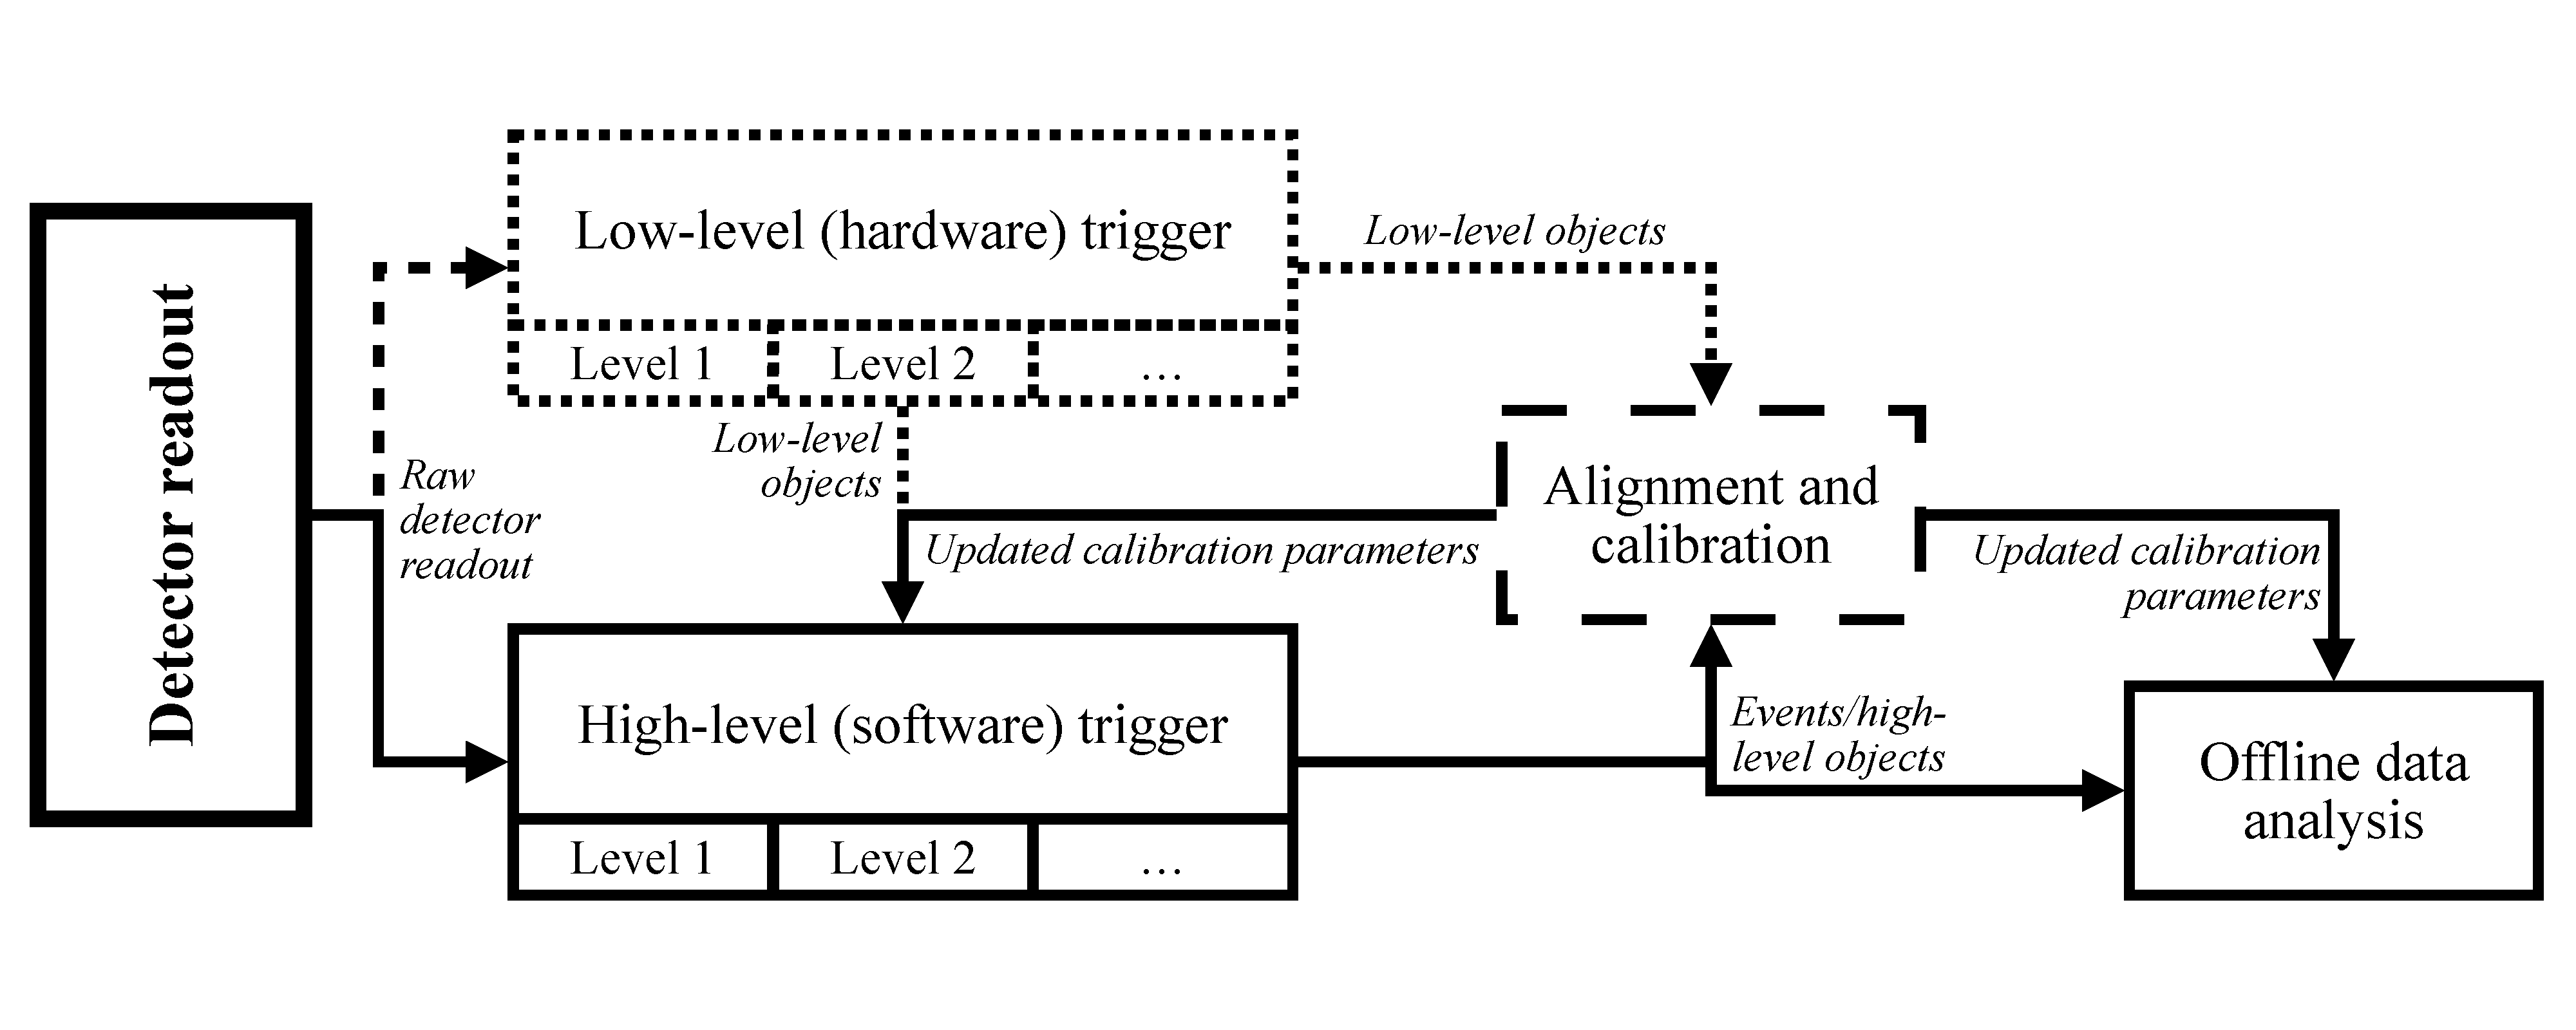
\includegraphics[width=\linewidth]{images/trigger_schematic.pdf}
    \caption[A generalised schematic of a trigger system for a HEP experiment in the current paradigm. Raw data is read out from each subdetector. A low-level (hardware) trigger is typically employed to synchronise readout and apply initial selection/compression algorithms. A high-level (software) trigger makes further selections on reconstructed objects of increasing accuracy, which are then saved for offline analysis. Alignment and calibration are often performed alongside the high-level trigger to inform the reconstruction algorithms required for detailed selections.]{A generalised schematic of a trigger system for an HEP experiment in the current paradigm. Raw data is read out from each subdetector. A low-level (hardware) trigger is typically{\protect\footnotemark} employed to synchronise readout and apply initial selection/compression algorithms. Low-level trigger information, and detector readout/reconstructed objects are combined in an event building stage. A high-level (software) trigger makes further selections on reconstructed objects of increasing accuracy, which are then saved for offline analysis. Alignment and calibration are often performed alongside the high-level trigger to inform the reconstruction algorithms required for detailed selections.}
    \label{trigger-schema}
\end{figure}
\footnotetext{LHCb does not employ a low-level trigger in Run~3~\cite{LHCb_upgrade_trigger_TDR} and the ALICE low-level trigger does not apply selection~\cite{alice-trigger-run3}.}


A low-level trigger must operate at a rate close to the collision rate of \SI{40}{\mega\hertz} and thus must have a minimal dead time between operations. The low-level trigger dead time can be reduced by operating at several stages, each of increasing latency, such that only the lowest-level, fastest operations must take place at the lowest latency level. However, even the highest latency levels of a low-level trigger generally require custom high-speed electronics to perform operations. The data processed by the low-level trigger, typically reduced in rate by a factor $\mathcal{O}\left(100\right)$, is then passed to the high-level trigger for more detailed processing.

High-level triggers must perform more complex and computationally intensive tasks such as event reconstruction and calibration. To ensure that such tasks can be performed at the low-level trigger output rate, the high-level trigger is usually separated into two tiers, with the first performing coarse reconstruction and initial selections requiring simpler reconstructed objects (e.g., tracks), and the second performing a detailed reconstruction for more complex selections. High-level triggers typically take the form of a computing farm, making use of parallel computing approaches to efficiently distribute tasks across the available computing resources.

The implementations of such systems in each of the major LHC experiments are introduced in the following sections.

%It is difficult to satisfy both the high efficiencies and high background rejection physics requirements, as well as the very small trigger latency to reduce dead time. Multi-trigger systems are usually introduced. The Level-1 (L1) Trigger is a hardware trigger, comprised of custom high-speed electronics, which makes decisions based off of coarsely reconstructed subset of information from the detector. The L1 trigger renders a selection decision every bunch crossing, with high signal efficiency and comparatively lower background rejection. The data harvested from the L1 trigger is typically more than experiment infrastructure can handle for permanent storage and offline data analysis. Therefore, more sophisticated software Higher Level Triggers (HLT) are usually implemented to further reduce the rate, using full-precision and finer granularity detector information. The maximum allowable acceptance rate L1 trigger is constrained by the detector read out, the speed of at which the HLT performs the more refined selection, and the rate at which the Data AcQuisition (DAQ) system can retrieve the data for permanent storage.  

%The DAQ bandwidth, which is determined by the available storage capabilities and computing power, is related to the maximum allowable trigger rate $R_{\mathrm{trigger}} ^ {max}$ as follows:

\subsection{Trigger systems of the ATLAS and CMS experiments}

The two general-purpose LHC experiments, ATLAS and CMS, have similar, broad physics programmes~\cite{ATLASMachine,collaboration2008cms}. In Run~3, these programmes include searches for new physics: indirectly, by probing the nature of known particles (e.g.,  the Higgs boson~\cite{snowmass-higgs}) at the precision frontier, and directly (e.g.,  through searches for dark matter candidates~\cite{snowmass-darkmatter}). Both experiments consist of concentric layered subdetectors; namely inner detectors for charged particle tracking, calorimeters for measurement of hadron/electromagnetically interacting particle energies and positions, and muon spectrometers for the identification and precise measurement of muons. Due to the wide variety of physics processes probed, the experiments contain a large number of detector channels, resulting in large event sizes of ${\sim}\SI{1}{\mega\byte}$. ATLAS and CMS implement similar two-tier trigger systems with a Level-1 (L1) hardware-based trigger and a software-based high-level trigger (HLT). In Run~2 and Run~3, the triggers of both experiments reduced the initial \SI{40}{\mega\hertz} bunch crossing rate to an L1 acceptance rate of \SI{100}{\kilo\hertz}, reduced further to a final HLT output rate of ${\sim}\SI{1}{\kilo\hertz}$. For average event sizes ranging from ${\sim}\SI{500}{\kilo\byte}$~\cite{ATLASRun3EventBuilder} to ${\sim}\SI{2}{\mega\byte}$~\cite{cmsRun3EventBuilder}, this corresponds to a HLT output bandwidth of $\mathcal{O}\left(\SI{1}{\giga\byte\per\second}\right)$.

\subsection{Trigger system of the LHCb experiment}

The LHCb experiment is a heavy-flavour experiment operating in the forward region, searching for new physics through precision studies of the properties of heavy-flavour decays, in particular CP- and flavour-violation. Following the upgrade of the detector prior to Run~3, the LHCb detector operates as a general-purpose forward detector. The LHCb trigger system was redesigned for Run~3, removing the low-level Level 0 (L0) hardware-based trigger previously employed in Runs 1 and 2. The simplistic cut on $p_{T}$ implemented in the L0 trigger could not discriminate between signal and background for hadronic signals, which would have resulted in a effeciency loss as seen in Fig. \ref{fig:LHCbL0TriggerYield}. As such, the LHCb trigger consists solely of a HLT, split between two stages: HLT1 and HLT2~\cite{Aaij:2019uij}. Following the removal of the L0 trigger, LHCb event readout has increased from \SI{1}{\mega\hertz} to \SI{30}{\mega\hertz}. During Run~2, HLT1 and HLT2 were decoupled to allow HLT1 to run synchronous to data-taking and HLT2 to run asynchronously, enabling  detector calibrations between the steps to improve reconstruction performance to offline quality~\cite{LHCb:Albrecht_2015}. 

\begin{figure}[h!]
    \centering
    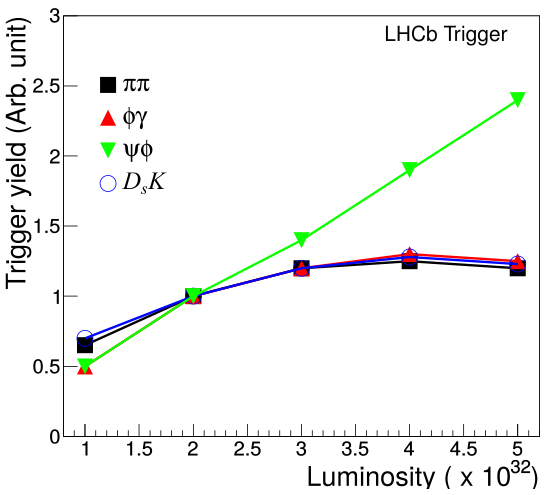
\includegraphics[width=0.55\linewidth]{images/lhcb/LHCb-L0-yield.png}
    \caption{Trigger yield per mode of interest with the Run 2 trigger configuration from Ref.~\cite{LHCb:upgrade-piucci}. Any increase in luminosity from accelerator upgrades is suppressed by the L0 trigger in all modes but $\psi\phi$ (i.e., non-muonic modes).}
    \label{fig:LHCbL0TriggerYield}
\end{figure}

HLT1 was upgraded throughout Run 2 to perform a partial reconstruction of the full detector readout. To achieve this, the reconstruction algorithm was upgraded to be able to run on GPUs hosted on the same event-building servers that host the FPGA cards required to receive data from the detector at 30 MHz~\cite{LHCb_Allen_GPU}. Reconstructed, selected events are propagated to a buffer at an event rate of ${\sim}\SI{1}{\mega\hertz}$. HLT2, implemented as a CPU farm known as the Event Filter Farm (EFF), takes as input the most recent detector alignment and calibration, reconstructing events in full offline quality for detailed selection. This selection reduces the event rate to \SI{100}{\kilo\hertz}, corresponding to an output bandwidth of \SI{10}{\giga\byte\per\second}~\cite{lhcb_hlt2_storage_run3}.

\subsection{Trigger system of the ALICE experiment}
The ALICE experiment is dedicated to the study of heavy-ion collisions at the LHC, with a focus on studies of quantum chromodynamics in energy-dense environments (e.g.,  quark-gluon plasma)~\cite{alice-performance-paper-run1}. To study such environments, ALICE studies p-p, p-Pb and Pb-Pb collisions at frequencies of \SI{1}{\mega\hertz}, \SI{500}{\kilo\hertz} and \SI{50}{\kilo\hertz}, respectively \cite{alice-trigger-run3}. Heavy ion collisions result in a very high multiplicity of particles, with ${\sim}\SI{700}{\mega\byte}$ of raw data per collision event collected by the ALICE experiment \cite{alice-rta-trigger}. The ALICE detector is barrel-shaped, containing concentric particle tracking and identification systems, and a forward muon spectrometer. At the core of the barrel is a Time Projection Chamber (TPC) vital to tracking performance, contributing the majority of the event size (\SI{95.3}{\percent} and \SI{91.1}{\percent} of total data volume in Pb-Pb and p-p collisions, respectively).

The ALICE trigger was upgraded ahead of Run~3 to facilitate continuous readout of subdetectors at collision frequency. The Central Trigger System (CTS), is responsible for the synchronisation of raw detector readout. The CTS transmits aggregated data and trigger signals to the HLT. The HLT then performs event reconstruction, data volume reduction and subdetector calibration, processing data at a maximum rate of \SI{48}{\giga\byte\per\second} to achieve an output throughput of up to \SI{12}{\giga\byte\per\second}~\cite{alice-rta-trigger}.
